\documentclass[12pt]{article}
\usepackage{graphicx}

\setlength{\oddsidemargin}{ 20pt}
\setlength{\textwidth}{440pt}
\setlength{\topmargin}{ 0pt}
\setlength{\headheight}{00pt}
\setlength{\headsep}{40pt}
\setlength{\textheight}{620pt}

\title {ENEE631 Assignment 3}
\author{Naotoshi Seo, sonots@umd.edu}
\date{February 28, 2007}


\begin{document}

\maketitle

\section{DCT basis images}

\subsection{Matlab Code}

\subsubsection{gen\_dctbasic.m}
\begin{verbatim}
function C = gen_dctbasis(N)
% Generate Basis Vectors for Unitary DCT
%
%  [C] = gen_dctbasis(N)
%
% Input arguments ([]s are optional):
%  N  (scalar) size N. 
%
% Output arguments ([]s are optional):
%  C  (matrix) of size NxN. Basis Vectors. Rows of C form orthonormal
%  basis.
%
% see also: dctmtx
%
% Author: Naotoshi Seo <sonots(at)umd.edu>
% Date  : March 2007
k = 0;
for n = 0:N-1
    C(k+1, n+1) = sqrt(1/N) * cos( pi*k*(2*n+1) / (2*N) );
end
for k = 1:N-1
    for n = 0:N-1
        C(k+1, n+1) = sqrt(2/N) * cos( pi*k*(2*n+1) / (2*N) );
    end
end
\end{verbatim}

\subsubsection{demo\_dctbasic.m}

\begin{verbatim}
function demo_dctbasis
% (1) 8x8 DCT Basis Images
%
%  demo_dctbasis
%
% Author: Naotoshi Seo <sonots(at)umd.edu>
% Date  : March 2007
N = 8;
C = gen_dctbasis(N);
B = gen_basisimages(C);
% plot
space = 2;
mini = min(min(min(min(B(:, :, :, :)))));
TILE = ones((N+space)*N, (N+space)*N) * mini;
for k = 0:N-1
    sk = k*(N+space)+1;
    for n = 0:N-1
        sn = n*(N+space)+1;
        TILE(sk:(sk+N-1), sn:(sn+N-1)) = B(:, :, k+1, n+1);
    end
end
imshow(TILE, 'DisplayRange', [min(min(TILE)) max(max(TILE))], ...
    'InitialMagnification', 300);
colorbar;
title('8x8 DCT basis images');
end

function B = gen_basisimages(C)
% Generate Basis Images associated with Input Basis Vectors
%
%  B = gen_basisimages(C)
%
% Input arguments ([]s are optional):
%  C  (matrix) of size NxN. Basis Vectors. Rows of C are orthonormal basis.
%
% Output arguments ([]s are optional):
%  B  (matrix) of size NxNx(NxN). Basis Images
%
% see also: gen_dctbasis, demo_dctbasis
%
% Author: Naotoshi Seo <sonots(at)umd.edu>
% Date  : March 2007
N = size(C, 1);
for n = 0:N-1
    for k = 0:N-1
        X = zeros(N, N);
        X(k+1, n+1) = 1;
        Y = C*X*C';
        B(:, :, k+1, n+1) = Y;
    end
end
end
\end{verbatim}

\subsection{Results and Observations}

\begin{center}
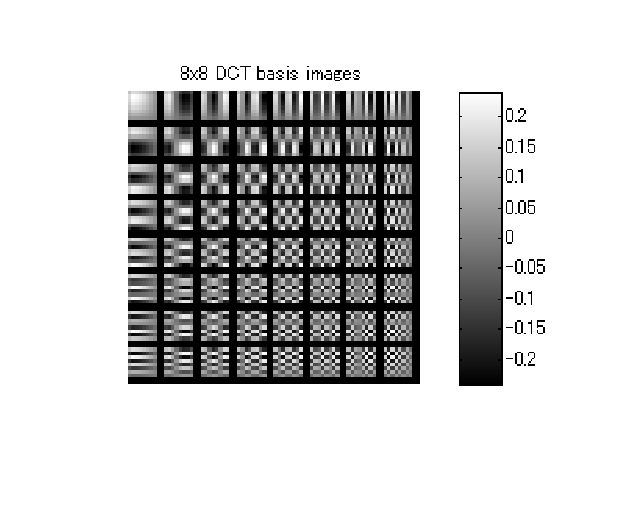
\includegraphics{../images/II1DCTBasisImage.eps}
\end{center}

\subsubsection{What are the characteristics of the basis image at the upper left corner?}

It was a constant, gray scale image. This means the most rough (coarse) approximation of the image, or low-pass filter. 

\subsubsection{How about the one at lower right corner?}

This image had fine blocks. This means that this basis expresses details, or high-pass filter. 

\newpage

\section{2-D DCT transform of images}

\subsection{Matlab Code}

\subsubsection{doDCT2.m}

\begin{verbatim}
function O = doDct2(I)
% 2-D Discrete cosine transform (DCT).
%
%  [O] = doDct2(I)
%
% Input arguments ([]s are optional):
%  I  (matrix) of size NxN. Input Image
%
% Output arguments ([]s are optional):
%  O  (matrix) of size NxN. Output Image
%
% Future Work: Support NxM image
%
% see also: dct2
%
% Author: Naotoshi Seo <sonots(at)umd.edu>
% Date  : March 2007
N = size(I, 1);
C = gen_dctbasis(N);
O = C*I*C';
\end{verbatim}

\subsubsection{doIDct2.m}

\begin{verbatim}
function O = doIDct2(I)
% 2-D Inverse Discrete cosine transform (Inverse DCT).
%
%  [O] = doIDct2(I)
%
% Input arguments ([]s are optional):
%  I  (matrix) of size NxN. Input Image
%
% Output arguments ([]s are optional):
%  O  (matrix) of size NxN. Output Image
%
% Future Work: Support NxM image
%
% see also: idct2
%
% Author: Naotoshi Seo <sonots(at)umd.edu>
% Date  : March 2007
N = size(I, 1);
C = gen_dctbasis(N);
O = C'*I*C;
\end{verbatim}

\subsubsection{demo\_dct2.m}

\begin{verbatim}
function demo_dct2
% (2) 2-D DCT Transform of images:
%
%  demo_dct2
%
% Author: Naotoshi Seo <sonots(at)umd.edu>
% Date  : March 2007

% Apply DCT to mysq.tif
mysq = double(imread('../images/mysq.tif'));
dctimg0 = doDct2(mysq);
figure;
imshow(log(abs(dctimg0)), [-1 12], 'InitialMagnification', 1500);
colormap(gray);
colorbar;
title('2-D DCT of mysq.tif');

% IDCT, Data Compression (Approximation) Test
N = size(mysq, 1);
for m = [1 2 4 8]
    reduced = zeros(N,N);
    reduced(1:m,1:m) = dctimg0(1:m,1:m);
    im = doIDct2(reduced);
    figure;
    imshow(im, [min(min(im)) max(max(im))], 'InitialMagnification', 1500);
    title(['DCT Data Compression Test m=',num2str(m),' ' ...
            num2str(floor(100*(m*m)/(N*N))), '%']);
end

% 2-D DCT for saturn image using built-in dct2 function
saturn = imread('../images/saturn.tif');
dctimg = dct2(saturn);
figure;
imshow(log(abs(dctimg)),[-1 12])
colormap(jet);
colorbar;
title('2-D DCT of saturn.tif');
\end{verbatim}

\subsection{2-D DCT on mysq.tif}

\begin{center}
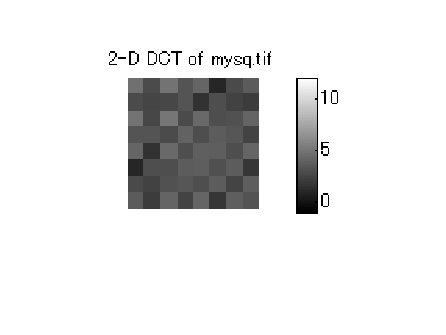
\includegraphics{../images/II2dctimg0.eps}
\end{center}

\subsection{2-D Inverse DCT - Data Compression Test}

\subsection{Results and Observations}

\begin{center}

\includegraphics{../images/II2IDCT1.eps}\\

\includegraphics{../images/II2IDCT2.eps}\\
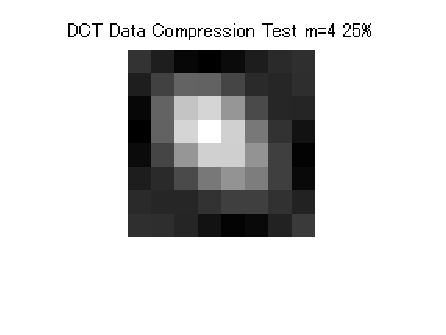
\includegraphics{../images/II2IDCT4.eps}\\
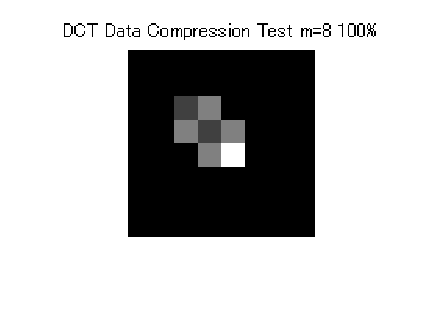
\includegraphics{../images/II2IDCT8.eps}\\
\end{center}

\subsubsection{Compare the four images and describe your observations}

The m = 1 image shows average of the input image. 
As increasing m, we obtained details and m = 8 gave (almost) perfect reconstruction. 

\subsubsection{Explain the results from the basis image point of view}

The upper left basis images give us approximation, and the lower right basis images give us details. 
As increasing m, we obtain basis images which express details, therefore, the obtained reconstructed images became finer as m increased. 

(By the way, we may be able to obtain derivative-like results by using only the lower right basis images. )


\subsection{2-D DCT on saturn.tif}

\begin{center}
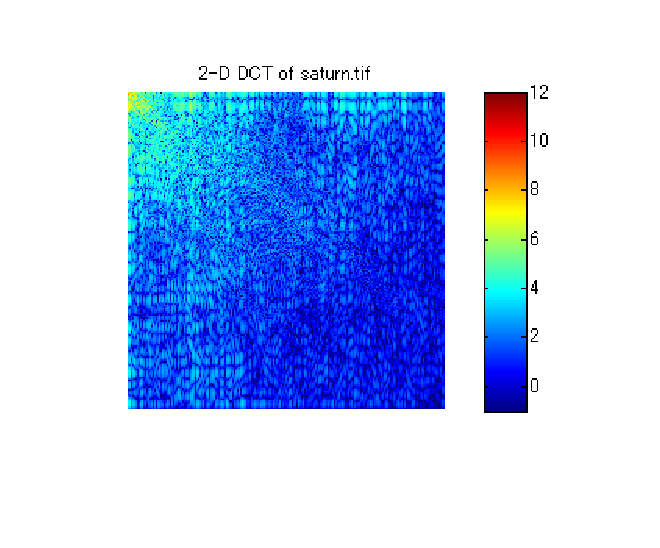
\includegraphics{../images/II2dctimg.eps}
\end{center}

\section{Block-based DCT transform of saturn image}

\subsection{Matlab Code}

\subsubsection{block\_dct2.m}

\begin{verbatim}
function O = block_dct2(I, m)
% Block Based 2-D DCT.
%
%  [O] = block_dct2(I, m)
%
% Input arguments ([]s are optional):
%  I   (matrix) of size NxN. Input Image
%  [m] (scalar): block size. Default is 8.
%
% Output arguments ([]s are optional):
%  O   (matrix) of size NxN. Output Image
%
% Future Work: 
%  Currently N must be a multiple of block size m. 
%  Support NxM image
%
% see also: blkproc, dct2
%
% Author: Naotoshi Seo <sonots(at)umd.edu>
% Date  : March 2007
if nargin < 2,
    m = 8;
end
N = size(I, 1);
for i=0:(floor(N/m)-1)
    si = i*m+1;
    for j=0:(floor(N/m)-1)
        sj = j*m+1;
        O(si:(si+m-1), sj:(sj+m-1)) = dct2(I(si:(si+m-1), sj:(sj+m-1)));
    end
end
\end{verbatim}

\subsubsection{demo\_block\_dct2.m}

\begin{verbatim}
function demo_block_dct2
% (3) Block-based DCT transform
%
%  demo_block_dct2
%
% Author: Naotoshi Seo <sonots(at)umd.edu>
% Date  : March 2007
saturn = imread('../images/saturn.tif');
blkdctimg = block_dct2(saturn);
figure;
imshow(log(abs(blkdctimg)),[-1 12])
colormap(jet);
colorbar;
title('Block-based 2-D DCT of saturn.tif');
\end{verbatim}

\subsection{Results and Observations}

\begin{center}
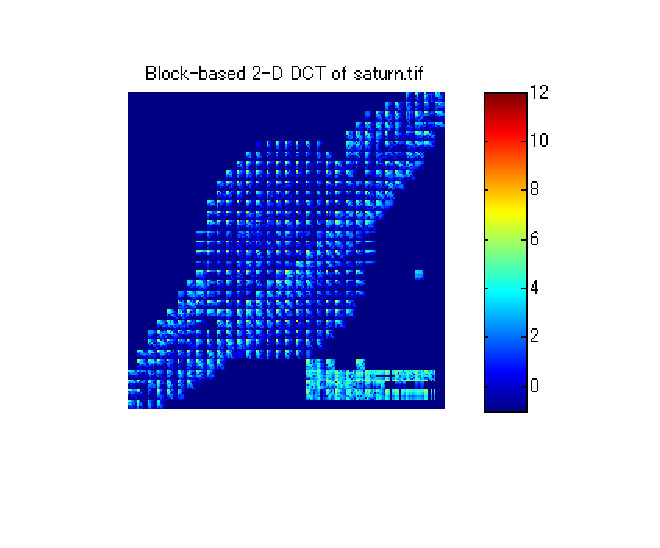
\includegraphics{../images/II3blkdctimg.eps}
\end{center}

\subsubsection{Compare blkdctimg with dctimg and discuss the difference}

We can see the shape of saturn in blkdctimg unlike in dctimg.  
This means the block based DCT retains the space information, too unlike DCT. 

\section{JPEG Experiment}
\subsection{Standard Mode}

\begin{center}
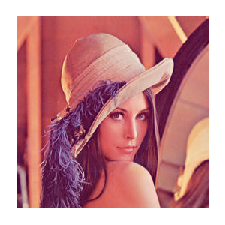
\includegraphics{../images/III1LenaC20.eps}\\
Compression factor 20 \\ 
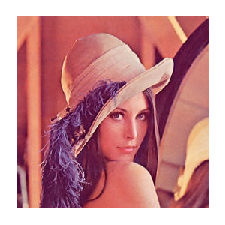
\includegraphics{../images/III1LenaC20r.eps}\\
Compression factor 20 with artifact removal\\
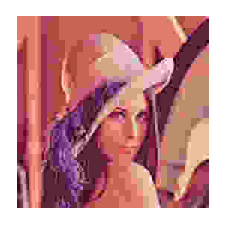
\includegraphics{../images/III1LenaC90.eps}\\
Compression factor 90 \\
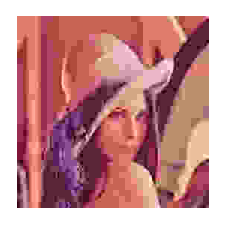
\includegraphics{../images/III1LenaC90r.eps}\\
Compression factor 90 with artifact removal\\
\end{center}

\subsubsection{Discuss the relationship between the compression factor and the image quality}

As compression factor increases, the image quality decreases. 

\subsubsection{Describe the artifacts caused by the 8x8 blocks}

As compression factor increases, the artifact became clearer. 
The block based DCT applies DCT to each small block, therefore, it has a drawback that it may result in visible artifacts. 

\subsection{Progressive mode}

\subsubsection{Observe how these images are loaded and displayed}

The progressive image, wash-irprog.jpg was first blurry (coarsely) displayed and then filled clearly. 
This filling was from the top to the bottom. 
The sequantial mode image was displayed clear from the first, from the top to the bottom. 

\section{Design a JPEG-like Codec}

\subsection{Matlab Codes}

\subsubsection{gen\_zigzagind.m}

\begin{verbatim}
function ind = gen_zigzagind(N)
% Generate zigzag association indices between matrix and to be generate
% vector for JPEG like zigzag scanning
%
%  ind = gen_zigzagind(N)
%
% Input arguments ([]s are optional):
%  N   (scalar) size of NxN matrix to be zigzag scanned
%
% Output arguments ([]s are optional):
%  ind (matrix) of size N^2x2. First column contains the appropriate row
%   indices and the second column contains the column indices of scanned matrix 
%
% Reference: 
%  JPEGtool collection of scripts for Octave and Matlab; 
%  http://www.dms.auburn.edu/compression
%
% Author: Naotoshi Seo <sonots(at)umd.edu>
% Date  : March 2007
ind = zeros(N,2);
c = 0;
r = 2;
increment = 1;
for n = 1:N*N
  r = r - increment; c = c + increment;
  if (c > N)
    r = r + 2; c = N; increment = -1;
  elseif (r < 1)
    r = 1; increment = -1;
  elseif (r > N)
    c = c + 2; r = N; increment = 1;
  elseif (c < 1)
    c = 1; increment = 1;
  end
  ind(n,:) = [r c];
end
\end{verbatim}

\subsubsection{ZigzagMtx2Vector.m}

\begin{verbatim}
function V = ZigzagMtx2Vector(A, ind)
% JPEG like zigzag scanning of matrix of size NxN into a vector
%
%  V = ZigzagMtx2Vector(A)
%
% Input arguments ([]s are optional):
%  A     (matrix) of size NxN.
%  [ind] (matrix) of size N^2x1. Zigzag indicies matrix if available
%
% Output arguments ([]s are optional):
%  V   (vector) of size 1xN^2
%
% see also: gen_zigzagind.m
%
% Author: Naotoshi Seo <sonots(at)umd.edu>
% Date  : March 2007
[nRow,nCol]=size(A);
if nRow ~= nCol
    error('input array should have equal number of rows and columns')
end
if nargin < 2,
    ind = gen_zigzagind(nRow); 
end
V = [];
for k=1:size(ind,1)
    V = horzcat(V, A(ind(k,1),ind(k,2)) ) ;
end
\end{verbatim}

\subsubsection{Vector2ZigzagMtx.m}

\begin{verbatim}
function A = Vector2ZigzagMtx(V, ind)
% JPEG like inverse zigzag scanning
%
%  A = Vector2ZigzagMtx(V)
%
% Input arguments ([]s are optional):
%  V     (vector) of size 1xN^2
%  [ind] (matrix) of size N^2x1. Zigzag indicies matrix if available
%
% Output arguments ([]s are optional):
%  A   (matrix) of size NxN. Restored matrix
%
% see also: gen_zigzagind.m
%
% Author: Naotoshi Seo <sonots(at)umd.edu>
% Date  : March 2007
if nargin < 2,
    ind = gen_zigzagind(sqrt(length(V))); 
end
A=[];
for k=1:length(V)
    A( ind(k,1),ind(k,2) )=V(k);
end    
\end{verbatim}


\subsubsection{my\_JpegChrQuanTable.m}

\begin{verbatim}
function c=my_JpegChrQuanTable()
c=[
1	1	2	4	6	11	11	11;
1	1	2	4	8	11	11	11;
2	2	3	4	11	11	11	11;
4	4	4	5	11	11	11	11;
6	8	11	11	11	11	11	11;
11	11	11	11	11	11	11	11;
11	11	11	11	11	11	11	11;
11	11	11	11	11	11	11	11];       
\end{verbatim}

\subsubsection{my\_JpegLumQuanTable.m}

\begin{verbatim}
function c=my_JpegLumQuanTable()
c=[
1	1	1	1	1	2	3	3;
1	1	1	1	1	3	3	3;
1	1	1	1	2	3	3	3;
1	1	1	1	2	4	4	3;
1	1	3	4	4	6	6	4;
1	2	3	3	4	5	6	5;
2	3	4	4	5	6	6	5;
5	5	5	5	5	5	5	5];   
\end{verbatim}

\subsubsection{jpegenc.m}

\begin{verbatim}
function [Ylen Cblen Crlen] = jpegenc(I, m, s, CF, zigzag)
% JPEG-like encoder
%
%  jpegenc(I)
%
% Input arguments ([]s are optional):
%  I   (matrix) of size NxN. Input Image.
%  m   (scalar) block size of block based DCT. Default is 8.
%  s   (scalar) downsampling factor for Cb, Cr. Default is 2.
%  CF  (scalar) Compression factor (correlated to the quantization scale
%  factor)
%  zigzag (0 or 1): flag to use zigzag scannning. Default is 1 (use). 
%
% Output arguments ([]s are optional):
%  Ylen, Cblen, Crlen (scalar) compressed file length for Y, Cb, Cr components
%  respectively
%
% Future Work: 
%  Support NxM image
%
% Author: Naotoshi Seo <sonots(at)umd.edu>
% Date  : March 2007
if nargin < 5,
    zigzag = 1;
end
if nargin < 4,
    CF = 1;
end
if nargin < 3,
    s = 2;
end
if nargin < 2,
    m = 8;
end
[nRow, nCol, z] = size(I);
I = double(I);
% RGB to YCbCr
YCbCr = rgb2ycbcr(I);
Y = YCbCr(:, :, 1);
Cb = YCbCr(:, :, 2);
Cr = YCbCr(:, :, 3);
% downsample Cb, Cr
dCb = imresize(Cb, 1/s);
dCr = imresize(Cr, 1/s);
% block based DCT
dctmat = dctmtx(m);
YDCT = blkproc(Y, [m m], 'P1*x*P1''', dctmat); % or 'dct2(x)'
dCbDCT = blkproc(dCb, [m m], 'P1*x*P1''', dctmat);
dCrDCT = blkproc(dCr, [m m], 'P1*x*P1''', dctmat);
fprintf('DCT done\n');
% quantization table
lumtable = my_JpegLumQuanTable*CF;
chrtable = my_JpegChrQuanTable*CF;
YDCTQuan = blkproc(YDCT,[m m],'round(x./P1)', lumtable);
dCbDCTQuan = blkproc(dCbDCT,[m m],'round(x./P1)', chrtable);
dCrDCTQuan = blkproc(dCrDCT,[m m],'round(x./P1)', chrtable);
fprintf('quantization done\n');
% zigzag scanning for each block
ind = gen_zigzagind(m);
YDCTQuanVec = [];
for j=0:(floor(nCol/m)-1)
    sj = j*m+1;
    for i=0:(floor(nRow/m)-1)
        si = i*m+1;
        if zigzag
            YDCTQuanVec = [YDCTQuanVec; ZigzagMtx2Vector(YDCTQuan(si:(si+m-1), sj:(sj+m-1)), ind)];
        else
            YDCTQuanVec = [YDCTQuanVec; reshape(YDCTQuan(si:(si+m-1), sj:(sj+m-1)), 1, m*m)];
        end
    end
end
dCbDCTQuanVec = [];
dCrDCTQuanVec = [];
for j=0:(floor(nCol/s/m)-1)
    sj = j*m+1;
    for i=0:(floor(nRow/s/m)-1)
        si = i*m+1;
        if zigzag
            dCbDCTQuanVec = [dCbDCTQuanVec; ZigzagMtx2Vector(dCbDCTQuan(si:(si+m-1), sj:(sj+m-1)), ind)];
            dCrDCTQuanVec = [dCrDCTQuanVec; ZigzagMtx2Vector(dCrDCTQuan(si:(si+m-1), sj:(sj+m-1)), ind)];
        else
            dCbDCTQuanVec = [dCbDCTQuanVec; reshape(dCbDCTQuan(si:(si+m-1), sj:(sj+m-1)), 1, m*m)];
            dCrDCTQuanVec = [dCrDCTQuanVec; reshape(dCrDCTQuan(si:(si+m-1), sj:(sj+m-1)), 1, m*m)];
        end
    end
end
fprintf('zigzag done\n');
% entropy encoding
Ylen = JPEG_entropy_encode(nRow, nCol, m, lumtable, YDCTQuanVec, '', 1);
path = 'Y_';
copyfile('JPEG.jpg', strcat(path, 'JPEG.jpg'));
copyfile('JPEG_DCTQ_ZZ.txt', strcat(path, 'JPEG_DCTQ_ZZ.txt'));
Cblen = JPEG_entropy_encode(nRow/s, nCol/s, m, chrtable, dCbDCTQuanVec, '', 1);
path = 'Cb_';
copyfile('JPEG.jpg', strcat(path, 'JPEG.jpg'));
copyfile('JPEG_DCTQ_ZZ.txt', strcat(path, 'JPEG_DCTQ_ZZ.txt'));
Crlen = JPEG_entropy_encode(nRow/s, nCol/s, m, chrtable, dCrDCTQuanVec, '', 1);
path = 'Cr_';
copyfile('JPEG.jpg', strcat(path, 'JPEG.jpg'));
copyfile('JPEG_DCTQ_ZZ.txt', strcat(path, 'JPEG_DCTQ_ZZ.txt'));
fprintf('entropy encoding done\n');
\end{verbatim}

\subsubsection{jpegdec.m}

\begin{verbatim}
function O = jpegdec(zigzag)
% JPEG-like  decoder
%
%  [O] = jpegenc
%
% Input arguments ([]s are optional):
%  zigzag (0 or 1): flag to use zigzag scannning. Default is 1 (use). 
%
% Output arguments ([]s are optional):
%  O   (matrix) of size NxN. Decoded Image
%
% Future Work: 
%  Support NxM image
%
% Author: Naotoshi Seo <sonots(at)umd.edu>
% Date  : March 2007
if nargin < 1,
    zigzag = 1;
end
% entropy decoding and load propeties
path = 'Cr_';
copyfile(strcat(path, 'JPEG.jpg'), 'JPEG.jpg');
copyfile(strcat(path, 'JPEG_DCTQ_ZZ.txt'), 'JPEG_DCTQ_ZZ.txt');
[nr, nc, m, chrtable, dCrDCTQuanVec] = JPEG_entropy_decode('');
path = 'Cb_';
copyfile(strcat(path, 'JPEG.jpg'), 'JPEG.jpg');
copyfile(strcat(path, 'JPEG_DCTQ_ZZ.txt'), 'JPEG_DCTQ_ZZ.txt');
[nc, nr, m, chrtable, dCbDCTQuanVec] = JPEG_entropy_decode('');
path = 'Y_';
copyfile(strcat(path, 'JPEG.jpg'), 'JPEG.jpg');
copyfile(strcat(path, 'JPEG_DCTQ_ZZ.txt'), 'JPEG_DCTQ_ZZ.txt');
[nRow, nCol, m, lumtable, YDCTQuanVec] = JPEG_entropy_decode('');
% m block size
s = nRow / nc; % down-up sampling factor;
% izigzag scanning for each block
ind = gen_zigzagind(m);
nBlock = size(YDCTQuanVec, 1);
nBlockInRow = floor(nRow / m);
for k=0:(nBlock-1)
    i = mod(k, nBlockInRow);
    j = floor(k / nBlockInRow);
    si = i*m+1;
    sj = j*m+1;
    if zigzag
        YDCTQuan(si:(si+m-1), sj:(sj+m-1)) = Vector2ZigzagMtx(YDCTQuanVec(k+1, :), ind);
    else
        YDCTQuan(si:(si+m-1), sj:(sj+m-1)) = reshape(YDCTQuanVec(k+1, :), m, m);
    end
end
nBlock = size(dCbDCTQuanVec, 1);
nBlockInRow = floor(floor(nRow / s) / m);
for k=0:(nBlock-1)
    i = mod(k, nBlockInRow);
    j = floor(k / nBlockInRow);
    si = i*m+1;
    sj = j*m+1;
    if zigzag
        dCbDCTQuan(si:(si+m-1), sj:(sj+m-1)) = Vector2ZigzagMtx(dCbDCTQuanVec(k+1, :), ind);
        dCrDCTQuan(si:(si+m-1), sj:(sj+m-1)) = Vector2ZigzagMtx(dCrDCTQuanVec(k+1, :), ind);
    else
        dCbDCTQuan(si:(si+m-1), sj:(sj+m-1)) = reshape(dCbDCTQuanVec(k+1, :), m, m);
        dCrDCTQuan(si:(si+m-1), sj:(sj+m-1)) = reshape(dCrDCTQuanVec(k+1, :), m, m);
    end
end
% inverse quantization table
YDCT = blkproc(YDCTQuan,[m m],'x.*P1', lumtable);
dCbDCT = blkproc(dCbDCTQuan,[m m],'x.*P1', chrtable);
dCrDCT = blkproc(dCrDCTQuan,[m m],'x.*P1', chrtable);
% inverse DCT
dctmat = dctmtx(m);
Y = blkproc(YDCT, [m m], 'P1''*x*P1', dctmat); % or 'idct2(x)'
dCb = blkproc(dCbDCT, [m m], 'P1''*x*P1', dctmat);
dCr = blkproc(dCrDCT, [m m], 'P1''*x*P1', dctmat);
% upsampling
Cb = imresize(dCb, s);
Cr = imresize(dCr, s);
% RGB to YCbCr
Y = uint8(Y + 128);
Cb = uint8(Cb + 128);
Cr = uint8(Cr + 128);
YCbCr = cat(3, Y, Cb, Cr);
O = ycbcr2rgb(YCbCr);
\end{verbatim}

\subsubsection{demo\_jpegcodec.m}

\begin{verbatim}
function demo_jpegcodec
    I = imread('../images/LenaC.bmp');
    jpegenc(I);
    O = jpegdec;
    imwrite(O, '../images/IIIJpegCodec.png');
    figure;
    imshow(O);
end
\end{verbatim}

\subsection{Results}

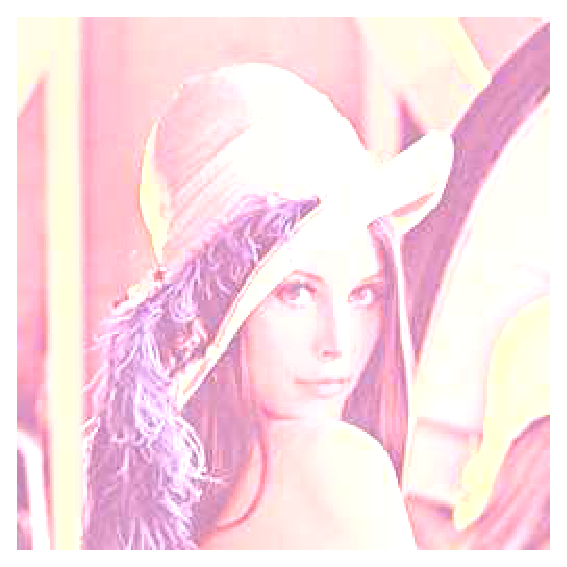
\includegraphics{../images/IIIJpegCodec.eps}

\section{Peak Signal-to-Noise Ratio vs Compression Ration}

\subsection{Matlab Code}

\subsubsection{psnr.m}

\begin{verbatim}
function [psnr] = psnr(I, O)
% Peak Signal-to-Noise Ratio of luminance components
%
%  psnr = psnr(I, O)
%
% Input arguments ([]s are optional):
%  I   (matrix) of size NxN. Original Image
%  O   (matrix) of size NxN. Code-decoded Image
%
% Output arguments ([]s are optional):
%  psnr (scalar) Peak Signal-to-Noise Ratio
%
% Author: Naotoshi Seo <sonots(at)umd.edu>
% Date  : March 2007
I = rgb2ycbcr(I);
IY = I(:, :, 1);
IY = double(IY);
O = rgb2ycbcr(O);
OY = O(:, :, 1);
OY = double(OY);
[nRow, nCol] = size(IY);
MSE = 0;
for i=1:nRow
    for j=1:nCol
        MSE = MSE+(IY(i,j)-OY(i,j))^2;
    end
end
MSE=MSE/(nRow*nCol);
psnr=10*log10(255^2./MSE);
\end{verbatim}

\subsubsection{demo\_plotpsnr.m}

\begin{verbatim}
function demo_plotpsnr
% Plot Peak Signal-to-Noise Ratio of luminance components in y-axis vs.
% Compression Ration (CR) in x-axis.
%  
%  demo_plotpsnr
%
% Input arguments ([]s are optional):
%  I   (matrix) of size NxN. Original Image
%  O   (matrix) of size NxN. Code-decoded Image
%
% Output arguments ([]s are optional):
%  psnr (scalar) Peak Signal-to-Noise Ratio
%
% Author: Naotoshi Seo <sonots(at)umd.edu>
% Date  : March 2007

I = imread('../images/LenaC.bmp');
% with zigzag scanning
[nRow nCol nColor] = size(I);
for i=1:5
    [Ylen Cblen Crlen] = jpegenc(I, 8, 2, i);
    O = jpegdec;
    PSNR(i) = psnr(I, O);
    CR(i) = (nRow * nCol) / Ylen;
end
figure;
plot(CR, PSNR);

% without zigzag scanning
for i=1:5
    [Ylen Cblen Crlen] = jpegenc(I, 8, 2, i, 0);
    O = jpegdec;
    PSNR(i) = psnr(I, O);
    CR(i) = (nRow * nCol) / Ylen;
end
figure;
plot(CR, PSNR);
end
\end{verbatim}

\subsection{Results and Observations}

\begin{center}
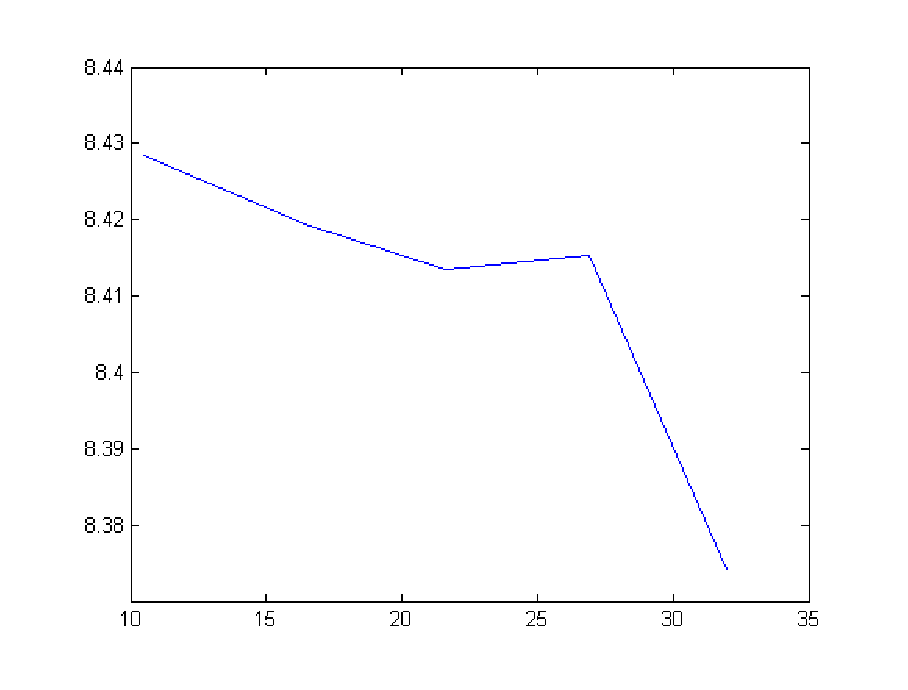
\includegraphics{../images/III2CRvsPSNR.eps}\\
with zigzag scan\\
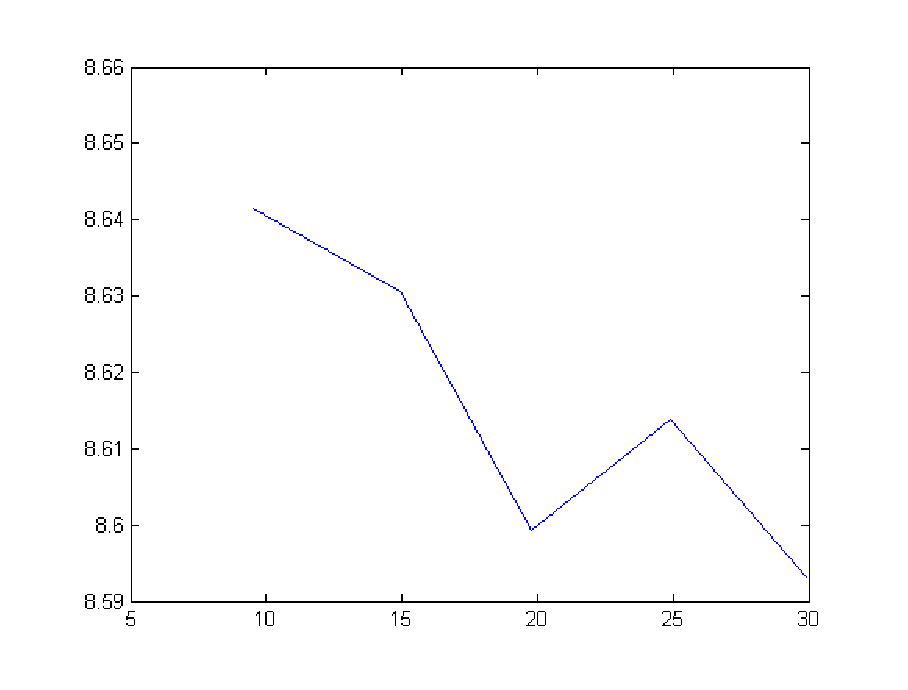
\includegraphics{../images/III2CRvsPSNRNoZigzag.eps}\\
without zigzag scan\\
\end{center}

\subsubsection{Discuss the advantage of zigzag scanning}

High frequencies in DCT basis image tends to be zero or less than zero. 
In 2-D DCT, we have horizontal and vertical frequncies, and therefore, scanning from upper left into lower right achieves better run-length coding gain.

\subsubsection{Compare the result with zigzag scanning and without zigzag scanning}

As shown, zigzag scanning version obtained higher PSNR than non-zigzag scanning version. 


\end{document}
